\documentclass[a4paper]{article}
\usepackage[utf8]{inputenc}
\usepackage[spanish, es-tabla]{babel}

\usepackage[a4paper, footnotesep = 1cm, width=18cm, left=2cm, top=2.5cm, height=25cm, textwidth=18cm, textheight=25cm]{geometry}
%\geometry{showframe}

\usepackage{amsmath}
\usepackage{amsfonts}
\usepackage{amssymb}
\usepackage{float}
\usepackage{graphicx}
\usepackage{caption}
\usepackage{subcaption}
\usepackage{multicol}
\usepackage{multirow}
\setlength{\doublerulesep}{\arrayrulewidth}

\usepackage{hyperref}
\hypersetup{
    colorlinks=true,
    linkcolor=blue,
    filecolor=magenta,      
    urlcolor=blue,
    citecolor=blue,    
}

\newcommand{\quotes}[1]{``#1''}
\usepackage{array}
\newcolumntype{C}[1]{>{\centering\let\newline\\\arraybackslash\hspace{0pt}}m{#1}}
\usepackage[american]{circuitikz}
\usepackage{fancyhdr}
\usepackage{units} 

\pagestyle{fancy}
\fancyhf{}
\lhead{22.11 Electrónica I}
\rhead{Mechoulam, Lambertucci, Rodriguez, Londero}
\rfoot{Página \thepage}

\begin{document}

%%%%%%%%%%%%%%%%%%%%%%%%%
%		Caratula		%
%%%%%%%%%%%%%%%%%%%%%%%%%

\begin{titlepage}
\newcommand{\HRule}{\rule{\linewidth}{0.5mm}}
\center
\mbox{\textsc{\LARGE \bfseries {Instituto Tecnológico de Buenos Aires}}}\\[1.5cm]
\textsc{\Large 22.11 Electrónica I}\\[0.5cm]


\HRule \\[0.6cm]
{ \Huge \bfseries Trabajo práctico N$^{\circ}$1}\\[0.4cm] 
\HRule \\[1.5cm]


{\large

\emph{Grupo 3}\\
\vspace{3px}

\begin{tabular}{lr} 	
\textsc{Mechoulam}, Alan  &  58438\\
\textsc{Lambertucci}, Guido Enrique  & 58009 \\
\textsc{Rodriguez Turco}, Martín Sebastian  & 56629 \\
\textsc{Londero Bonaparte}, Tomás Guillermo  & 58150 \\
\end{tabular}

\vspace{20px}

\emph{Profesores}\\
Alcocer, Fernando\\
Oreglia, Eduardo Victor\\
Gardella, Pablo Jesús\\
\vspace{3px}
%\textsc{} \\	

\vspace{100px}

\begin{tabular}{ll}

Presentado: & 24/09/19\\

\end{tabular}

}

\vfill

\end{titlepage}


%%%%%%%%%%%%%%%%%%%%%
%		Indice		%
%%%%%%%%%%%%%%%%%%%%%

\tableofcontents
\newpage

%%%%%%%%%%%%%%%%%%%%%
%		Informe		%
%%%%%%%%%%%%%%%%%%%%%
\section{Introducción}
En el siguiente informe se busca analizar, desarrollar y confeccionar un circuito amplificador con componentes discretos utilizando de base lo aprendido a lo largo del cuatrimestre. Se destaca la existencia de una dificultad adicional, la cual se basa en el método mediante el cual se fueron adquiriendo los componentes. Estos fueron subastados durante la cursada, entre los diversos grupos. De esta forma, se condiciona el circuito final, ya que se posee acceso limitado a los recursos, los cuales no se pudieron elegir libremente.

\section{Componentes dispuestos}
El presente grupo se valió de los siguientes componentes:
\begin{itemize}
	\item Dos pares de resistencias de $6.8 \ k\Omega$ y de $680 \ k\Omega$.
	\item Un transistor BJT NPN. 
	\item Un diodo 1N4148.
	\item Un JFET.
	\item Un par Darlington NPN.
	\item Una placa de 5x5.
\end{itemize}

\section{Circuitos considerados}
Como primer opción se consideró utilizar el par Darlington y mediante el uso de las resistencias, configurarlo de forma tal que este quede compensado. Una alternativa es el uso de una fuente de corriente, con el mismo objetivo que se mencionó anteriormente.
\begin{figure}[H]
\centering
\begin{subfigure}{.45\textwidth}
\centering
	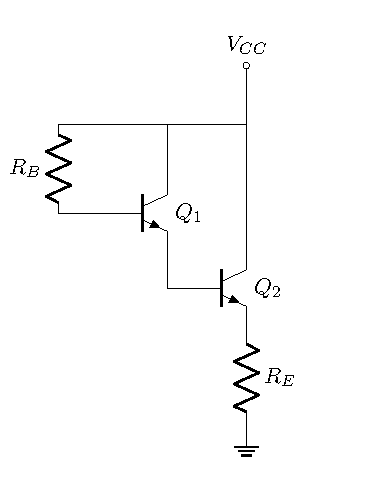
\includegraphics[width=0.5\textwidth, page=1]{Imagenes/ParDarlington.pdf}
	\caption{Par Darlington.}
	\label{fig:pardar1}
\end{subfigure}
\begin{subfigure}{.4\textwidth}
\centering
	\includegraphics[width=0.6\textwidth, page=2]{Imagenes/ParDarlington.pdf}
	\caption{Par Darlington compensado con $R$.}
	\label{fig:pardar2}
\end{subfigure}
\begin{subfigure}{.5\textwidth}
\centering
	\includegraphics[width=0.5\textwidth, page=3]{Imagenes/ParDarlington.pdf}
	\caption{Par Darlington compensado con fuente de corriente.}
	\label{fig:pardar3}
\end{subfigure}
\caption{Configuraciones y modificaciones posibles para el par Darlington.}
\label{fig:pardar}
\end{figure}

La conexión representada en la Figura (\ref{fig:pardar1}) no es la más conveniente. Una de las principales desventajas consiste en que si es deseable aumentar la ganancia de tensión del sistema, se debe modificar el valor de $R_E$, modificando también la polarización del sistema. En otras palabras, se debe realizar un balance adecuado y tener muy en cuenta lo que uno busca optimizar.

Por otro lado, la mostrada en la Figura (\ref{fig:pardar2}) permite aumentar la corriente $I_{CE1}$ y aprovecharla de cierta forma llevándola al colector de $Q_2$. Una variación que busca mejorar esta configuración consiste en colocar la resistencia a tierra, ya que de esta forma permite extraer más corriente de $Q_1$.

Finalmente, la mostrada en la Figura (\ref{fig:pardar3}) se considera la más óptima para compensar el circuito, ya que permite polarizar el transistor $Q_2$ mediante corriente, aprovechando también la resistencia a tierra mencionada para el caso anterior. Una particularidad de esta disposición es que la fuente empleada actúa tanto en la polarización como una carga activa. Además, de esta forma, es posible aumentar $I_{CE2}$ sin modificar otros factores del propio circuito.

Cabe aclarar que, la disposición presentada en la Figura (\ref{fig:pardar2}), estrictamente hablando, es la más económica al problema anterior. Dadas las condiciones, dicha consideración no afecta en la decisión a implementar, ya que se cuenta con componentes para realizar cualquiera de las tres.

\section{Fuente de corriente}
\label{sec:fdei}
Una vez determinado que la implementación óptima, con los componentes disponibles, es la presentada en la Figura~(\ref{fig:pardar3}), se decide llevar adelante su análisis y confeccionarla. Para ello, primero se opta por analizar la fuente de corriente. Esta puede ser realizada con el JFET, dispuesto en una configuración en la cual se autopolarice, como se presenta a continuación.
\begin{figure}[H]
\centering
	\includegraphics[width=0.25\textwidth, page=4]{Imagenes/ParDarlington.pdf}
	\caption{Fuente de corriente.}
	\label{fig:fuentei}
\end{figure}

\subsection{Polarización}
Recorriendo la malla de entrada del circuito de la Figura (\ref{fig:fuentei}), se obtiene la siguiente ecuación:
\begin{equation*}
	V_{GS} = V_{SS} - I_{DS} R_{S}
\end{equation*}
%\begin{equation}
%	V_{DS} = V_{DD} + V_{SS} - I_{D} \left( R_{D} + R_{S} \right)
%\end{equation}

Además, se plantean las ecuaciones del JFET:
\begin{equation*}
	I_{D} = I_{DSS} \left( 1 - \frac{V_{GS}}{V_P} \right)^2 \\
\end{equation*}
\begin{equation*}
	gm = \ 2\frac{\sqrt{I_{D} I_{DSS}}}{|V_P|}
\end{equation*}

De esta forma, seleccionando el componente \href{https://www.onsemi.com/pub/Collateral/2N3819-D.PDF}{2N3819}, se obtiene de la hoja de datos los valores de interés, tales como $I_{DSS} = 2 \ mA$ y $V_P = -8 \ V$, siendo estos los adecuados para el peor caso. Luego, estableciendo $V_{SS} = 10 \ V$, $R_g = 6.8 \ K\Omega$ y $R_D = 680 \ \Omega$ y operando algebraicamente, se calculan la corriente de drain y la tensión gate-source. Como es de esperarse, se obtienen dos valores posibles para cada variable:
\begin{equation*}
\left\lbrace
\begin{split}
	&I_{D} =  4.39 \ mA \\
	&V_{GS} =  -19.85 \ V
\end{split}
\right.
\ \ y \ \
\left\lbrace
\begin{split}
	&I_{D} =  1.60 \ mA \\
	&V_{GS} =  -0.88 \ V
\end{split}
\right.
\end{equation*}

\subsection{Impedancia de salida}
Sabiendo que se debe cumplir que $I_{DSS} \geq I_{D}$ y $V_{GS} > V_{P}$, se descartan los primeros valores, seleccionando $I_{D} = 1.60 \ mA$ y $V_{GS} = -0.88 \ V$, obteniéndose así $gm = 0.45 \ \frac{mA}{V}$. De esta forma se garantiza que esté polarizado adecuadamente.

Con lo establecido previamente, se prosigue a plantear el circuito incremental. Es de interés calcular la impedancia de salida, para luego reemplazar la configuración por dicha variable en el análisis incremental del circuito de la Figura~(\ref{fig:pardar3}). Esto se debe a que la fuente no sufre variaciones incrementales. Si esta fuese una fuente referencial, no se da la misma situación y no se podría efectuar lo previamente mencionado.
\begin{figure}[H]
\centering
	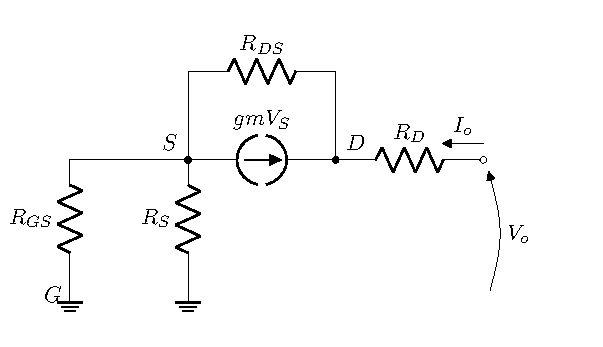
\includegraphics[width=0.5\textwidth, page=1]{Imagenes/ModeloIncremental.pdf}
	\caption{Circuito incremental de la Figura (\ref{fig:fuentei}).}
\label{fig:incfuente1}
\end{figure}

Se destaca que, como el gate queda a tierra, se cumple que $V_{GS} = V_G - V_S = - V_S$, por lo tanto, se da vuelta la fuente de corriente y se reemplaza con lo mencionado anteriormente. 

Se define $R_{GS}^* = R_S // R_{GS}$, para luego analizar el circuito presentado en la Figura (\ref{fig:incfuente2}).
\begin{figure}[H]
\centering
\hspace*{2cm}
	\includegraphics[width=0.45\textwidth, page=2]{Imagenes/ModeloIncremental.pdf}
	\caption{Análisis de la impedancia de salida del circuito de la fuente de corriente.}
\label{fig:incfuente2}
\end{figure}

Observando que la tensión $V_S$ es igual a $R_{GS}^{*} I_o$, planteando las corrientes del nodo $D$ y analizando la tensión $V_o$ se obtienen las siguientes ecuaciones:
\begin{equation}
	V_o = I_{D} R_{DS} + I_o \left( R_D + R_{GS}^* \right)
	\label{equ:riojfet1}
\end{equation}
\begin{equation}
	I_{D} = gm V_S + I_o = \left( gm R_{GS}^* + 1 \right) I_o
	\label{equ:riojfet2}
\end{equation}

Reemplazando con (\ref{equ:riojfet2}) en (\ref{equ:riojfet1}) y dividiendo miembro a miembro por $I_o$ , se obtiene la impedancia de entrada deseada.
\begin{equation}
\begin{split}
	R_{OF} & = \frac{V_o}{I_o} = R_{DS} \left( 1 + gm R_{GS}^* \right) + R_{GS}^* + R_D \\
		   & = R_{DS} \left( 1 + gm R_S//R_{GS} \right) + R_S//R_{GS} + R_D
\end{split}
\label{equ:rof}
\end{equation}

Para poder continuar, se toma $R_{GS} \longrightarrow \infty$ y se asume $V_A = -90 \ V$, ya que dicho valor no se encuentra en la hoja de datos y este puede asumirse para los peores casos. Luego, se estima $R_{DS} = \frac{V_A}{I_{D}} = 56.25 \ K\Omega$. De esta forma se obtiene de (\ref{equ:rof}) el valor de la impedancia de salida $R_{OF} \approx 234.79 \ K\Omega$.

\section{Darlington polarizado por corriente}
Con lo obtenido en la Sección (\ref{sec:fdei}), se posee la información necesaria para analizar el circuito presentado en la Figura (\ref{fig:pardar3}). En el análisis que se muestra a continuación se presentan la carga y la alimentación del sistema, componentes que no fueron presentados en la Figura (\ref{fig:pardar}) por cuestiones de simplicidad.
\begin{figure}[H]
\centering
	\includegraphics[width=0.5\textwidth, page=5]{Imagenes/ParDarlington.pdf}
	\caption{Circuito equivalente al reemplazar la fuente de corriente.}
	\label{fig:pardar4}
\end{figure}

\subsection{Polarización}
A continuación, se seleccionan los transistores a utilizar en el par Darlington, eligiendo \href{https://www.sparkfun.com/datasheets/Components/BC546.pdf}{BC547} para este caso. Por un lado, como se está polarizando este transistor por corriente, se garantiza que $I_{CE2} = 1.60 \ mA$. Por otro lado, para el caso de $Q_1$, se plantea la malla de entrada, obteniéndose así la corriente $I_{CQ1}$ de la forma
\begin{equation*}
	V_{CC} - I_{B1} R_B - V_{BEON} - \left( I_{CE1} - I_{B2} \right) R_E = 0
\end{equation*}
\begin{equation*}
	V_{CC} - V_{BEON} - I_{B2} R_E = I_{B1} R_B + I_{CE1} R_E = I_{CE1} \left( \frac{R_B}{h_{fe1}} + R_E \right)
\end{equation*}
\begin{equation}
	I_{CE1} = \left( V_{CC} - V_{BEON} + I_{CE2} \frac{R_E}{h_{FE2}} \right) \left( \frac{R_B}{h_{fe1}} + R_E \right)^{-1}
\end{equation}

Es así que, para la tensión $V_{CE1}$, se obtiene
\begin{equation}
	V_{CE1} = V_{CC} - I_{CE1} R_E
\end{equation}

Luego se recorre la malla que conecta $V_{CC}$ con el emisor de $Q_2$, pasando por las bases y emisores de ambos transistores. Llamando a la tensión en el emisor de $Q_2$ como $V_{DD}$, se obtiene
\begin{equation*}
	V_{CC} - I_{CE1} \frac{R_B}{h_{fe1}} - 2 V_{BEON} - V_{DD} = 0
\end{equation*}
\begin{equation}
	V_{DD} = V_{CC} - I_{CE1} \frac{R_B}{h_{fe1}} - 2 V_{BEON}
	\label{equ:vdd}
\end{equation}

Finalmente, recorriendo la malla de salida de $Q_2$, se llega a la ecuación
\begin{equation*}
	V_{CC} - V_{CE2} - V_{DD} = 0
\end{equation*}
\begin{equation}
	V_{CE2} = V_{CC} - V_{DD}
	\label{equ:vce2}
\end{equation}

Es así que, tomando $V_{CC} = 12 \ V$, $R_E = 680 \ \Omega$ y $R_B = 6.8 \ k\Omega$, se obtiene $I_{CE1} = 15.25 \ mA$, $V_{CE1} = 1.63 \ V$, $V_{DD} = 9.82 \ V$ y $V_{CE2} = 2.08 \ V$, teniendo así el transistor $Q_1$ polarizado.

Con lo analizado, mediante el uso de simulaciones e información del transistor obtenida de la hoja de datos, se cuenta la información necesaria para poder efectuar una aproximación a las rectas de carga estática y dinámica.
\begin{figure}[H]
\centering
	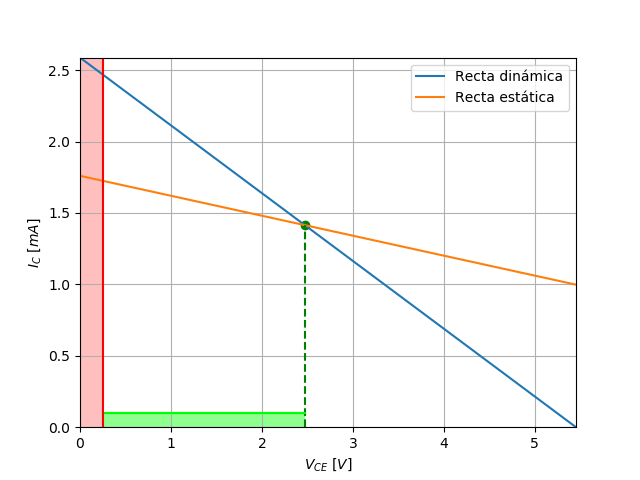
\includegraphics[width=0.5\textwidth]{Imagenes/RectaDeCarga.png}
	\caption{Recta de carga del circuito.}
\label{fig:rcarg}
\end{figure}

Sabiendo que la tensión de saturación del transistor es $V_{SAT} = 0.25 \ V$ en el peor caso, se presenta en la Figura (\ref{fig:rcarg}) la zona de saturación del transistor en rojo, mientras que en verde, se muestra la región del eje horizontal que representa la excursión simétrica máxima, la cual es limitada por el factor previamente mencionado. De esta forma, se calcula el valor del $ESM$, siendo este de $2.22 \ V$.

\subsection{Circuito incremental}
Asumiendo $T = 27^o C$ y $V_{A1} = V_{A2} = V_A = -90 \ V$ y sabiendo que los estimadores empleados son $gm = \frac{I_{CE}}{V_T}$, $h_{ie} = \frac{h_{fe}}{gm}$ y $\frac{1}{h_{oe}} = \frac{V_A}{I_{CE}}$, se buscan conseguir dichos valores para cada BJT. Para el caso de $h_{fe1}$ y $h_{fe2}$ se obtiene de la hoja de datos un valor de $h_{fe} = 200$, ya que se dispuso de integrado que cae en la clasificación tipo B. 

Con todos los datos obtenidos y presentados, se elabora la siguiente tabla, en la cual se presentan los valores de los estimadores necesarios.
\begin{table}[H]
\centering
\begin{tabular}{cccc}
\hline
\textbf{Transistor} & $\mathbf{gm \ \left[ \frac{mA}{V} \right]}$ & $\mathbf{h_{ie} \ \left[ K\Omega \right]}$ & $\mathbf{\frac{1}{h_{oe}} \ \left[ K\Omega \right]}$ \\
\hline
$Q_1$ & 589.90 & 0.34 & 5.90 \\
$Q_2$ & 61.89 & 3.23 & 56.25	\\
\hline
\end{tabular}
\caption{Estimadores y datos pertinentes del modelo incremental del circuito Darlington.}
\label{tab:estim}
\end{table}

El siguiente paso consiste en reemplazar la fuente de corriente por su respectiva impedancia de salida $R_{OF}$, ya que no sufre variaciones incrementales, como se mencionó anteriormente. Planteando su respectivo modelo incremental, se llega al circuito presentado a continuación: 
\begin{figure}[H]
\centering
	\includegraphics[width=0.85\textwidth, page=3]{Imagenes/ModeloIncremental.pdf}
	\caption{Circuito incremental del par Darlington.}
\label{fig:incdar}
\end{figure}

Se observa en la Figura (\ref{fig:incdar}) que se puede obtener una relación entre $I_{B2}$ e $I_o$, mediante el uso de un divisor de corriente, siendo esta
\begin{equation*}
	I_o = I_{B2} \left( 1 + h_{fe2} \right) \frac{R_{OF} // \frac{1}{h_{oe2}}}{R_L + R_{OF} // \frac{1}{h_{oe2}}}
\end{equation*}
\begin{equation}
	\frac{I_o}{I_{B2}} = \left( 1 + h_{fe2} \right) \frac{R_{OF} // \frac{1}{h_{oe2}}}{R_L + R_{OF} // \frac{1}{h_{oe2}}}
	\label{equ:io-ib2}
\end{equation}

Luego, definiéndose $R_{O1}^{*} = R_{E} // \frac{1}{h_{oe1}}$ y $R_d = R_{OF} // \frac{1}{h_{oe2}} // R_L$, se obtiene
\begin{figure}[H]
\centering
	\includegraphics[width=0.8\textwidth, page=4]{Imagenes/ModeloIncremental.pdf}
\end{figure}

Aplicando paso a nivel de corriente para la fuente de $h_{ie2} I_{B2}$, se llega a
\begin{figure}[H]
\centering
	\includegraphics[width=0.8\textwidth, page=5]{Imagenes/ModeloIncremental.pdf}
\end{figure}

Por un lado se destaca que 
\begin{equation*}
	V_o = I_{B2} R_d \left( 1 + h_{fe2} \right)
\end{equation*}
\begin{equation}
	\frac{V_o}{I_{B2}} = R_d \left( 1 + h_{fe2} \right)
\label{equ:vo-ib2}
\end{equation}

Por otro lado, se puede hallar una relación entre $I_{B1}$ e $I_{B2}$, de la misma forma que se realizó con $I_o$ e $I_{B2}$, siendo así
\begin{equation*}
	I_{B2} = I_{B1} \left( 1 + h_{fe1} \right) \frac{R_{O1}^{*}}{ R_{O1}^{*} + h_{ie2} + R_d \left( 1 + h_{fe2} \right) }
\end{equation*}
\begin{equation}
	\frac{I_{B2}}{I_{B1}} = \left( 1 + h_{fe1} \right) \frac{R_{O1}^{*}}{ R_{O1}^{*} + h_{ie2} + R_d \left( 1 + h_{fe2} \right) }
	\label{equ:ib2-ib1}
\end{equation}

De manera análoga, se toma el equivalente al paralelo entre $R_{O1}^{*}$ con $h_{ie2}$ y $R_d \left( 1 + h_{fe2} \right)$. Por lo tanto, se define $R_{d}^* = R_{O1}^{*} // \left[ h_{ie2} + R_d \left( 1 + h_{fe2} \right) \right]$ para luego aplicar paso a nivel de corriente con la segunda fuente.
\begin{figure}[H]
\centering
	\includegraphics[width=0.6\textwidth, page=6]{Imagenes/ModeloIncremental.pdf}
\end{figure}

De esta forma, se observa que
\begin{equation*}
	V_i = I_{B1} \left[ h_{ie1} + R_{d}^* \left( 1 + h_{fe1} \right) \right]
\end{equation*}
\begin{equation}
	\frac{V_i}{I_{B1}} = h_{ie1} + R_{d}^* \left( 1 + h_{fe1} \right)
	\label{equ:vi-ib1}
\end{equation}

Finalmente, se planteando nuevamente un divisor de corrientes, se obtiene
\begin{equation*}
	I_{B1} = I_i \frac{R_B}{R_B + h_{ie1} + R_{d}^* \left(1 + h_{fe1} \right)}
\end{equation*}
\begin{equation}
	\frac{I_{B1}}{I_i} = \frac{R_B}{R_B + h_{ie1} + R_{d}^* \left(1 + h_{fe1} \right)}
	\label{equ:ib1-ii}
\end{equation}

Con lo obtenido en (\ref{equ:vo-ib2}), (\ref{equ:ib2-ib1}) y (\ref{equ:vi-ib1}) y multiplicando, tanto el denominador como el numerador, por $I_{B1}$ e $I_{B2}$, se procede a calcular la transferencia $\Delta V$, siendo esta de la forma
\begin{equation}
	\Delta V \triangleq \frac{V_o}{V_i} = \frac{V_o}{I_{B2}} \frac{I_{B2}}{I_{B1}} \frac{I_{B1}}{V_i} = \frac{ \left( 1+h_{fe2} \right) R_d}{h_{ie2}+ \left( 1+h_{fe2} \right) R_d}
\label{equ:Av}
\end{equation}

De forma análoga, se calcula la ganancia de corriente. Utilizando (\ref{equ:io-ib2}), (\ref{equ:ib2-ib1}) y (\ref{equ:ib1-ii}), se obtiene
\begin{equation*}
	\Delta I \triangleq \frac{I_o}{I_i} = \frac{I_o}{I_{B2}} \frac{I_{B2}}{I_{B1}} \frac{I_{B1}}{I_i}
\end{equation*}
\begin{equation}
	\Delta I = \frac{R_C R_{O1}^{*} R_B \left( 1 + h_{fe2} \right) \left( 1+h_{fe1} \right)}{ \left( R_{OF} R_L h_{oe2} + R_{OF} + R_L \right)  \left\lbrace \left[ \left( 1 + h_{fe2} \right) \left( 1 + h_{fe1} \right) R_d + h_{fe1} h_{ie2} + R_B + h_{ie2} \right] R_{O1}^{*} + R_B \left[ h_{ie2} + \left( 1 + h_{fe2} \right) R_d \right]  \right\rbrace }
	\label{equ:Ai}
\end{equation}

Similar a los casos anteriores, se calcula la impedancia de entrada del amplificador, mediante el uso de (\ref{equ:vi-ib1}) y (\ref{equ:ib1-ii}). Reemplazando el sistema por su impedancia de entrada y aplicando un divisor de tensiones se llega a dicha expresión, siendo esta
\begin{equation}
	R_{ia} = \frac{V_i}{I_i} =  \frac{V_i}{I_{B1}}\frac{I_{B1}}{I_i} = \frac{ R_B R_{O1}^{*} \left[ h_{ie2} + \left( 1 + h_{fe2} \right) R_d \right] \left( 1 + h_{fe1} \right) }{ \left[ \left( 1 + h_{fe2} \right)  \left( 1 + h_{fe1} \right) R_d + h_{fe1} h_{ie2} + R_B + h_{ie2} \right] R_{O1}^{*} + R_B \left[ h_{ie2} + \left( 1 + h_{fe2} \right) R_d \right] }
	\label{equ:Ria}
\end{equation}

Una vez obtenidos $\Delta V$ y $R_{ia}$, se puede calcular la ganancia de tensión del sistema $\Delta V_S$, siendo esta
\begin{equation}
\begin{split}
	\Delta V_S \triangleq \frac{V_S}{V_i} = \frac{V_S}{V_o} \frac{V_o}{V_i} = \frac{V_o}{V_i} \frac{R_{ia}}{R_g + R_{ia}}
\end{split}
\label{equ:Avs}
\end{equation}

Por otro lado, para el cálculo de la impedancia de salida $R_{oa}$, se reemplaza la fuente $V_S$ por su impedancia de salida, considerándose el circuito de la siguiente forma:
\begin{figure}[H]
\centering
	\includegraphics[width=0.8\textwidth, page=7]{Imagenes/ModeloIncremental.pdf}
\end{figure}
Se definen $R_{g}^{*} = \left( R_B // R_g \right) + h_{ie1}$ y $R_{OF}^* = R_{OF} // \frac{1}{h_{oe1}}$. Luego, sabiendo que la tensión sobre $R_{O1}^{*}$ y $R_{g}^{*}$ es la misma, se obtiene
\begin{equation}
	I_{E}^{*} = I_{B1} \frac{R_{g}^{*}}{R_{O1}^{*}}
	\label{equ:roa1}
\end{equation}

Luego, observando el nodo $E_2$, se llega a
\begin{equation}
	\left[ I_{B2} \left( 1 + h_{fe2} \right) + I_o \right] R_{OF}^* = V_o
	\label{equ:roa2}
\end{equation}

Se expresa la tensión $V_o$ como
\begin{equation}
	V_o = - \left( I_{B1} h_{ie1} + I_{B2} h_{ie2} \right)
	\label{equ:roa3}
\end{equation}
y se plantea para el nodo $E_1$, utilizando (\ref{equ:roa1}), llegándose a la expresión
\begin{equation*}
	I_{B2} = I_{B1} \left( 1 +h_{fe1} + \frac{I_{S}^{*}}{I_{E}^{*}} \right)
\end{equation*}
\begin{equation}
	I_{B1} = \frac{I_{B2}}{1 +h_{fe1} + \frac{R_{g}^{*}}{R_{E}^{*}}}
	\label{equ:roa4}
\end{equation}

Reemplazando (\ref{equ:roa4}) en (\ref{equ:roa3}) se obtiene
\begin{equation}
	V_o = - I_{B2} \left( h_{ie2} + \frac{R_{g}^{*}}{ 1 +h_{fe1} + \frac{R_{g}^{*}}{R_{E}^{*}}} \right)
	\label{equ:roa5}
\end{equation}

Finalmente, con lo expresado en (\ref{equ:roa5}), al reemplazarlo en (\ref{equ:roa1}), se llega a
\begin{equation}
	\frac{V_o}{I_o} = \frac{R_{OF}}{h_{ie2} + \frac{R_{g}^{*}} {1 + h_{fe1} + \frac{R_{g}^{*}}{R_{E}^{*}}}  + R_{OF} \left( 1 + h_{fe2} \right)} \left( h_{ie2} + \frac{R_{g}^{*}} {1 + h_{fe1} + \frac{R_{g}^{*}}{R_{E}^{*}}}  \right)
	\label{equ:roa}
\end{equation}

Ya conseguidas las expresiones previas, solo resta reemplazar los valores de cada componente y estimador que permitan obtener el resultado final para cada una. Dichos valores son expresados en la Tabla (\ref{tab:resultados}).

\begin{table}[H]
\centering
\begin{tabular}{ccc}
\hline
\textbf{Variable} & \textbf{Valor} & \textbf{Valor en dB} \\
\hline
$\Delta V$ & 0.9897 & -0.0900 \\
$\Delta V_S$ & 0.9102 & -0.8140 \\
$\Delta I$ & 2.8853 & 9.2039 \\
$R_{ia}$ & 6.4430 $K\Omega$ & - \\
$R_{oa}$ & 16.0971 $\Omega$ & - \\
\hline
\end{tabular}
\caption{Valores obtenidos del circuito incremental.}
\label{tab:resultados}
\end{table}

Dado que la configuración elaborada consiste en dos transitores BJT dispuestos como colector común, es esperable poseer una ganancia de tensión del amplificador próxima a uno, al igual que una alta impedancia de entrada y baja de salida. El hehco de que la ganancia del sistema sea menor que uno también es esperable, ya que depende de la relación resultante del divisor resistivo entre $R_{ia}$ y $R_g$. El hecho de que $\Delta V_S$ se aleje de la cota máxima se debe a que $R_{ia}$ es simplemente un orden de magnitud mayor que $R_g$. Por otro lado, es sorprendente obtener una ganancia de corriente tan baja. Esto se analiza con mayor profundidad en al Sección (\ref{sec:conclusiones}).

\section{Desarrollo y armado de la placa}
Una vez realizado el calculo teórico, se realizó el circuito analizado. Primero, se presenta el PCB confeccionado mediante el uso del software \textbf{Altium}.
\begin{figure}[H]
\centering
	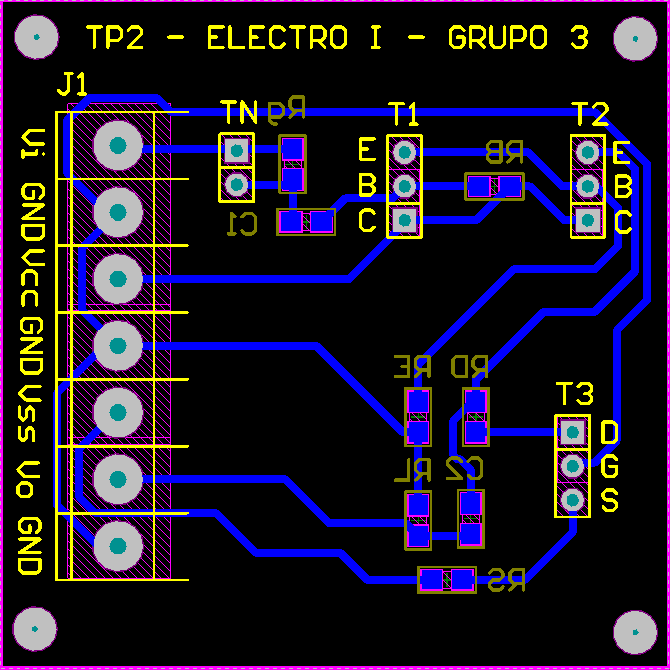
\includegraphics[width=0.3\textwidth]{Imagenes/PCB.png}
	\caption{PCB obtenido en Altium.}
\end{figure}

De esta forma, se procede a presentar las fotos del circuito elaborado.
\begin{figure}[H]
\centering
\begin{subfigure}{.49\textwidth}
\centering
	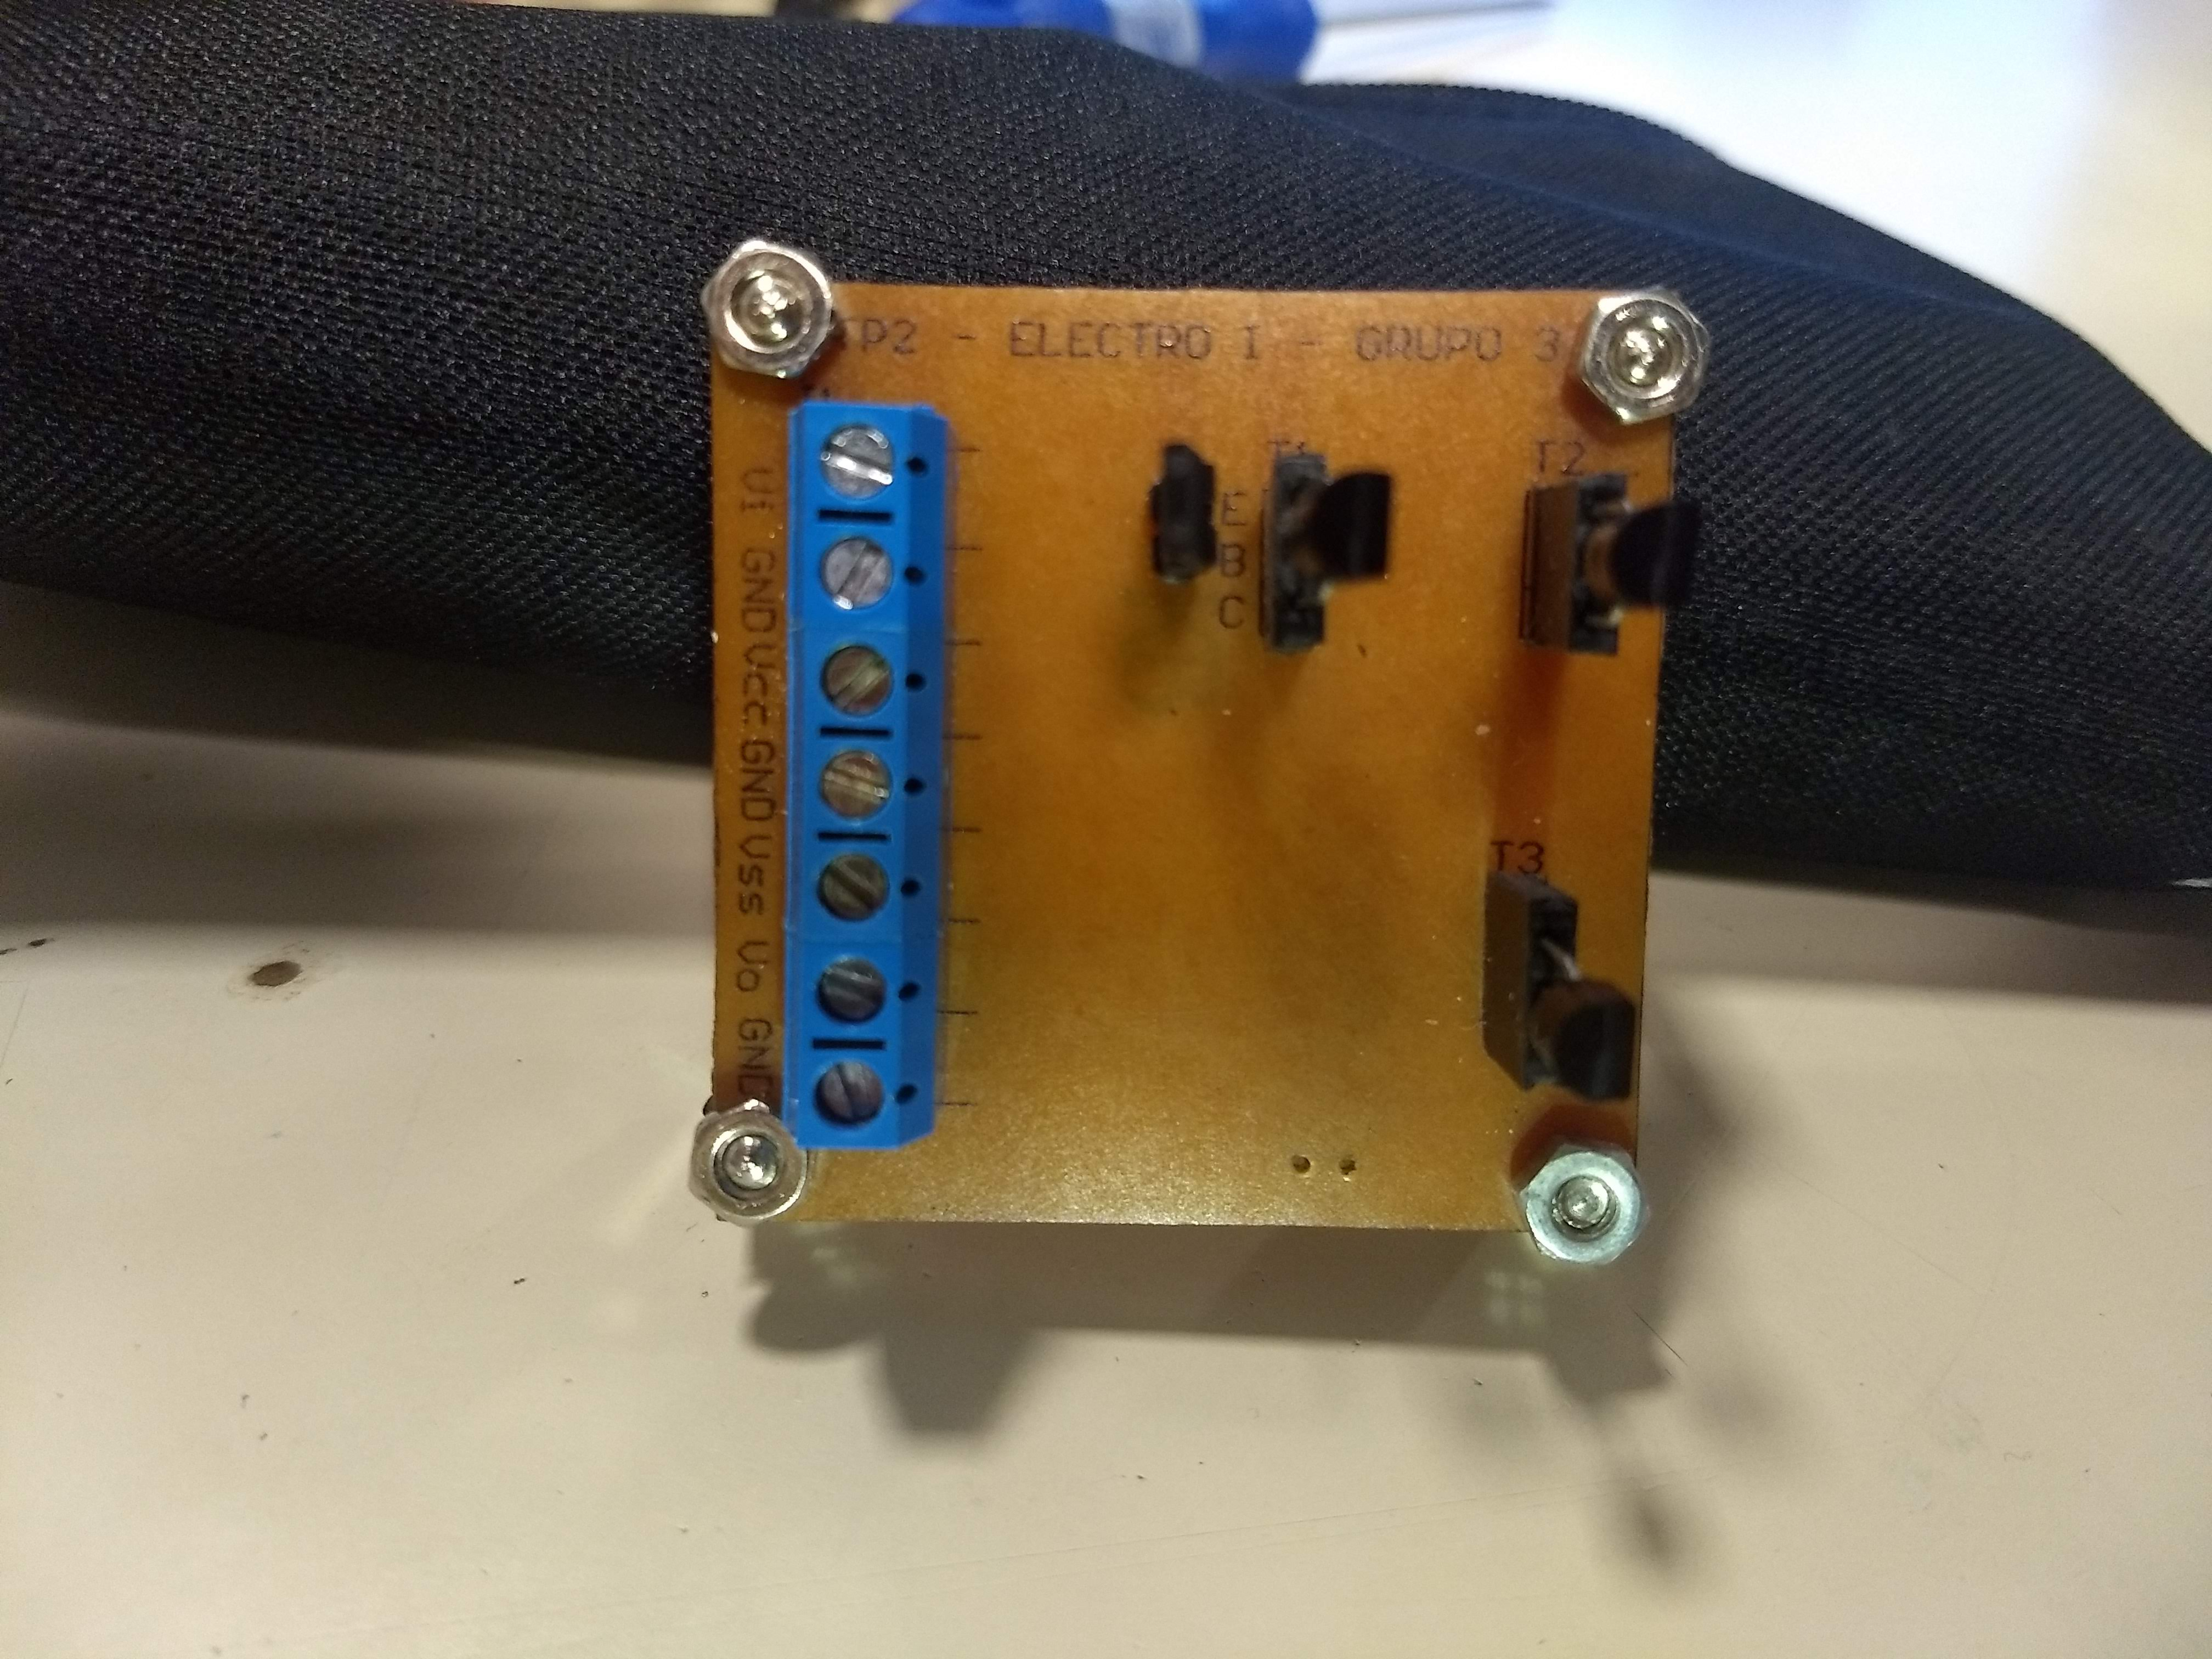
\includegraphics[width=0.6\textwidth, trim={40cm 20cm 30cm 15cm}, clip]{Imagenes/Placa-Up.jpg}
	\caption{Top Layer de la placa efectuada.}
	\label{fig:pup}
\end{subfigure}
\begin{subfigure}{.49\textwidth}
\centering
	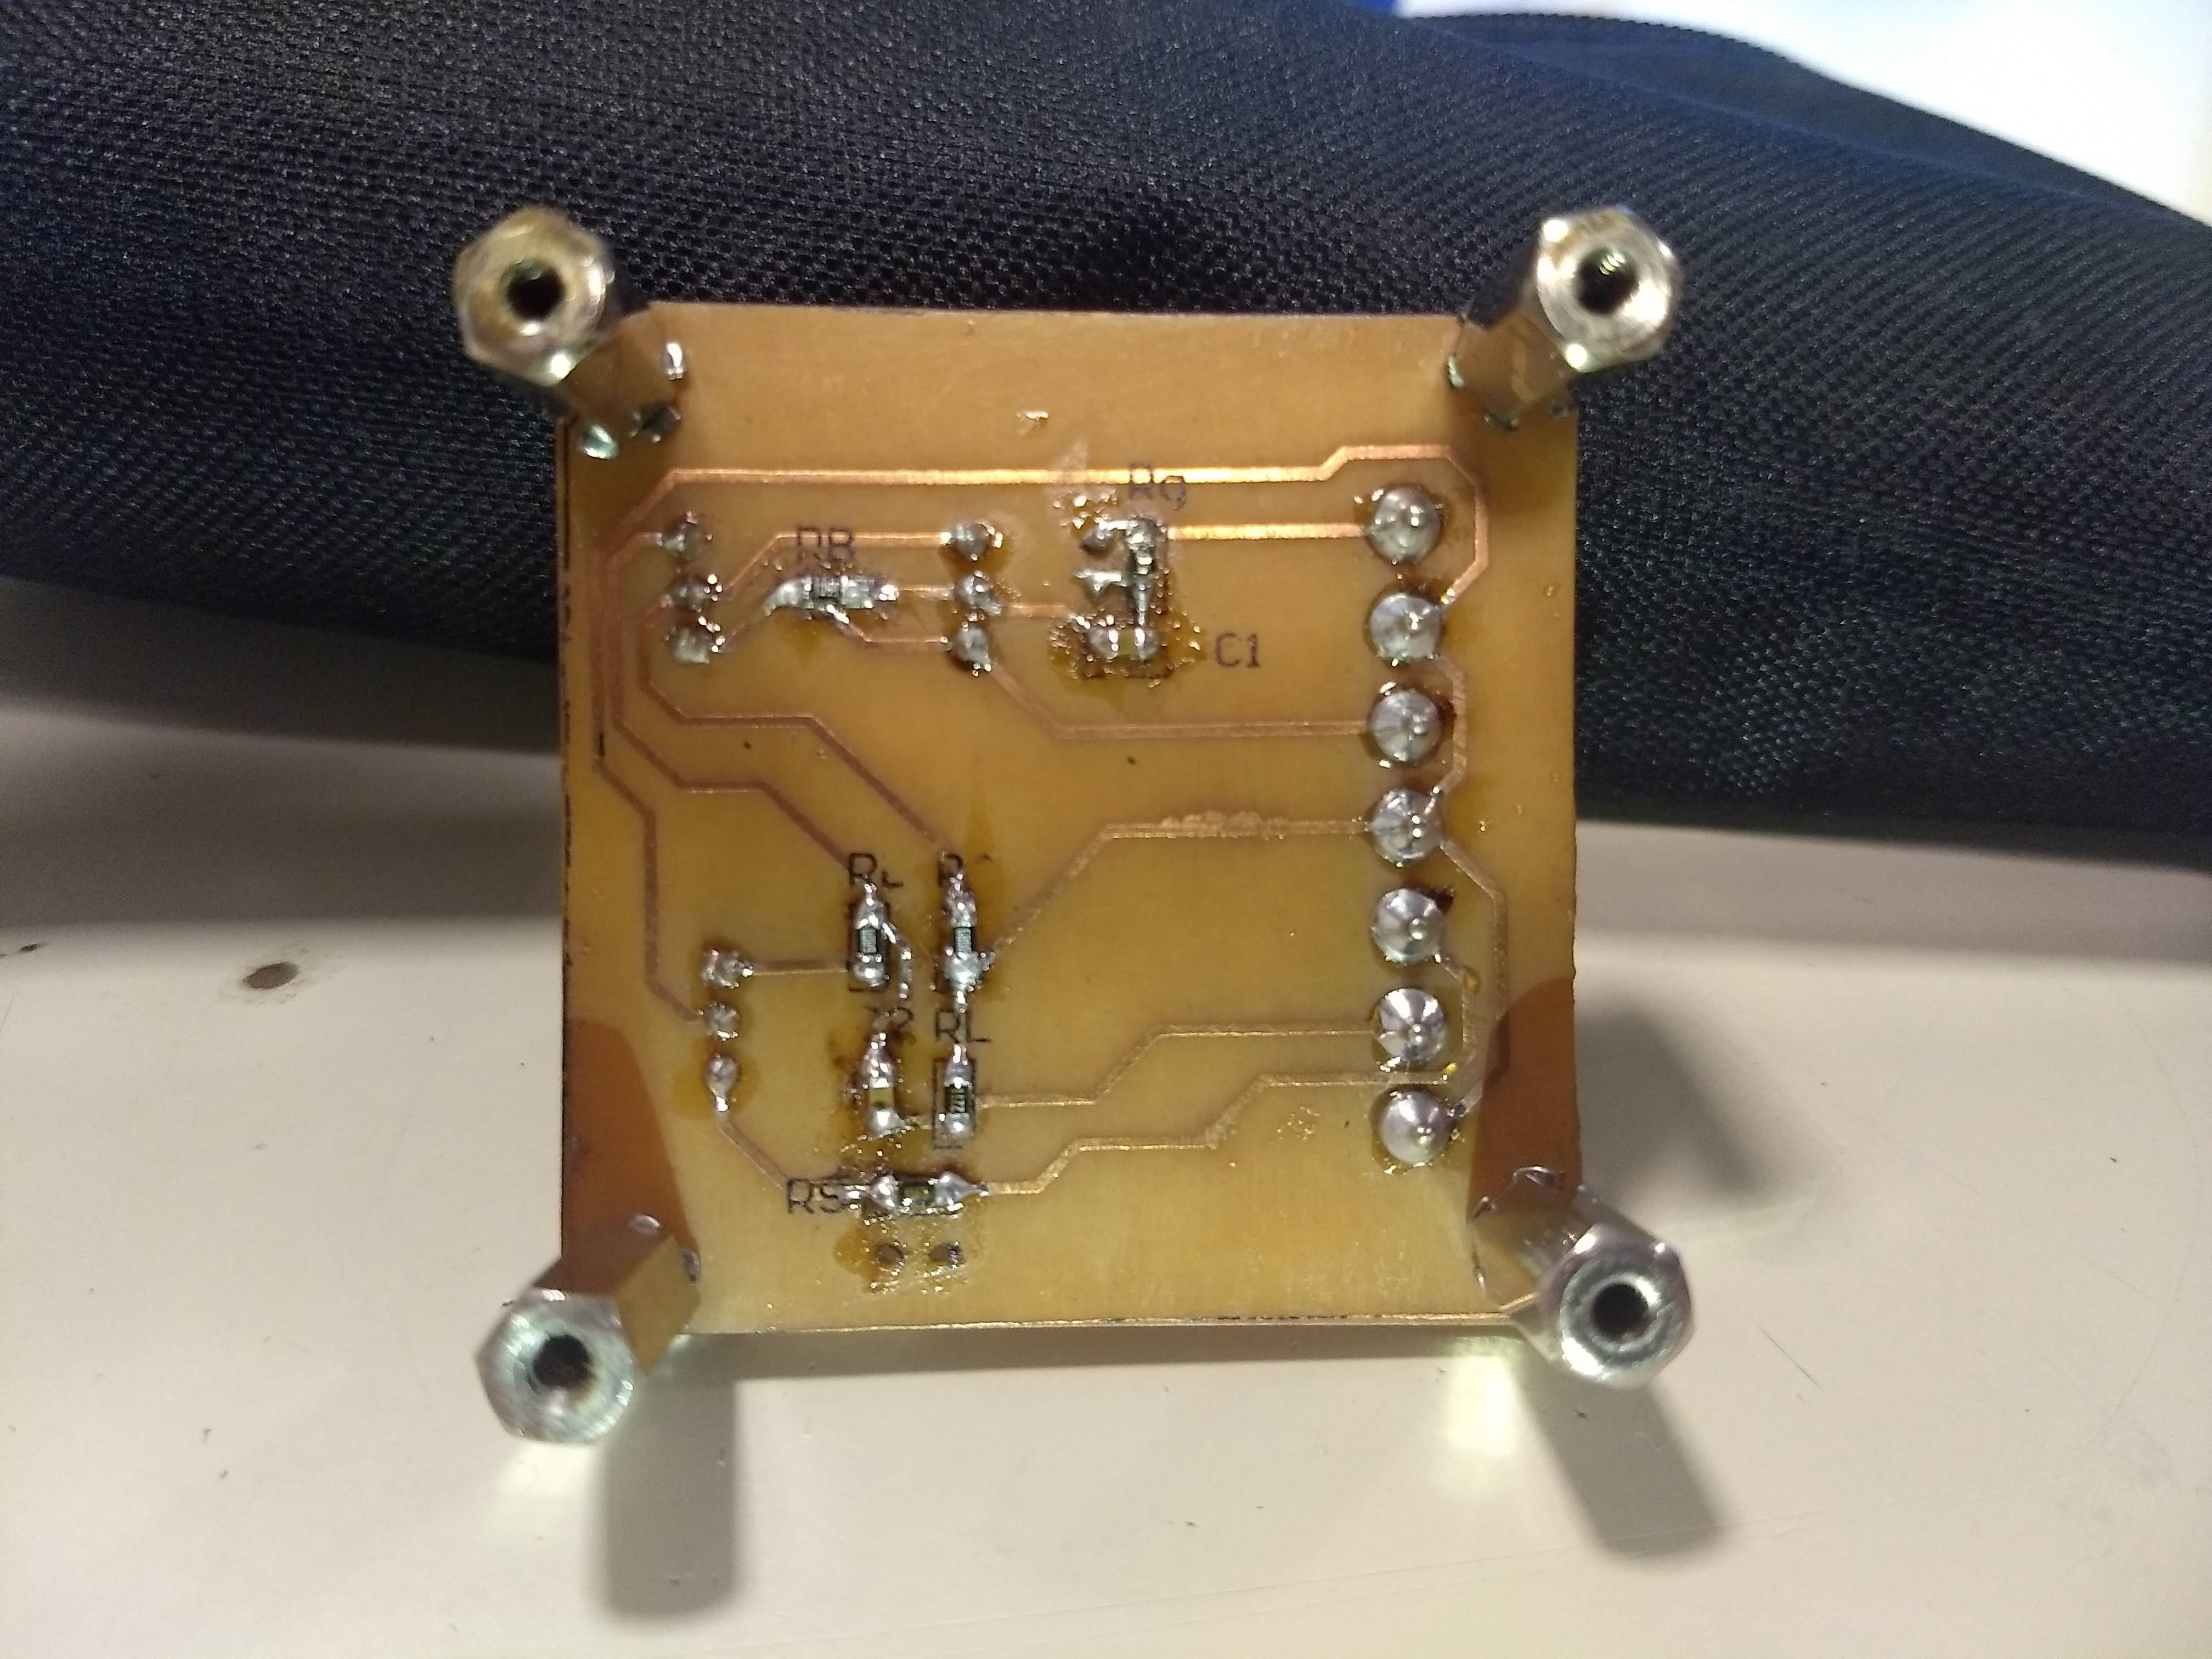
\includegraphics[width=0.6\textwidth, trim={25cm 10cm 30cm 10cm}, clip]{Imagenes/Placa-Down.jpg}
	\caption{Bottom Layer de la placa efectuada.}
	\label{fig:pd}
\end{subfigure}
\begin{subfigure}{.8\textwidth}
\centering
	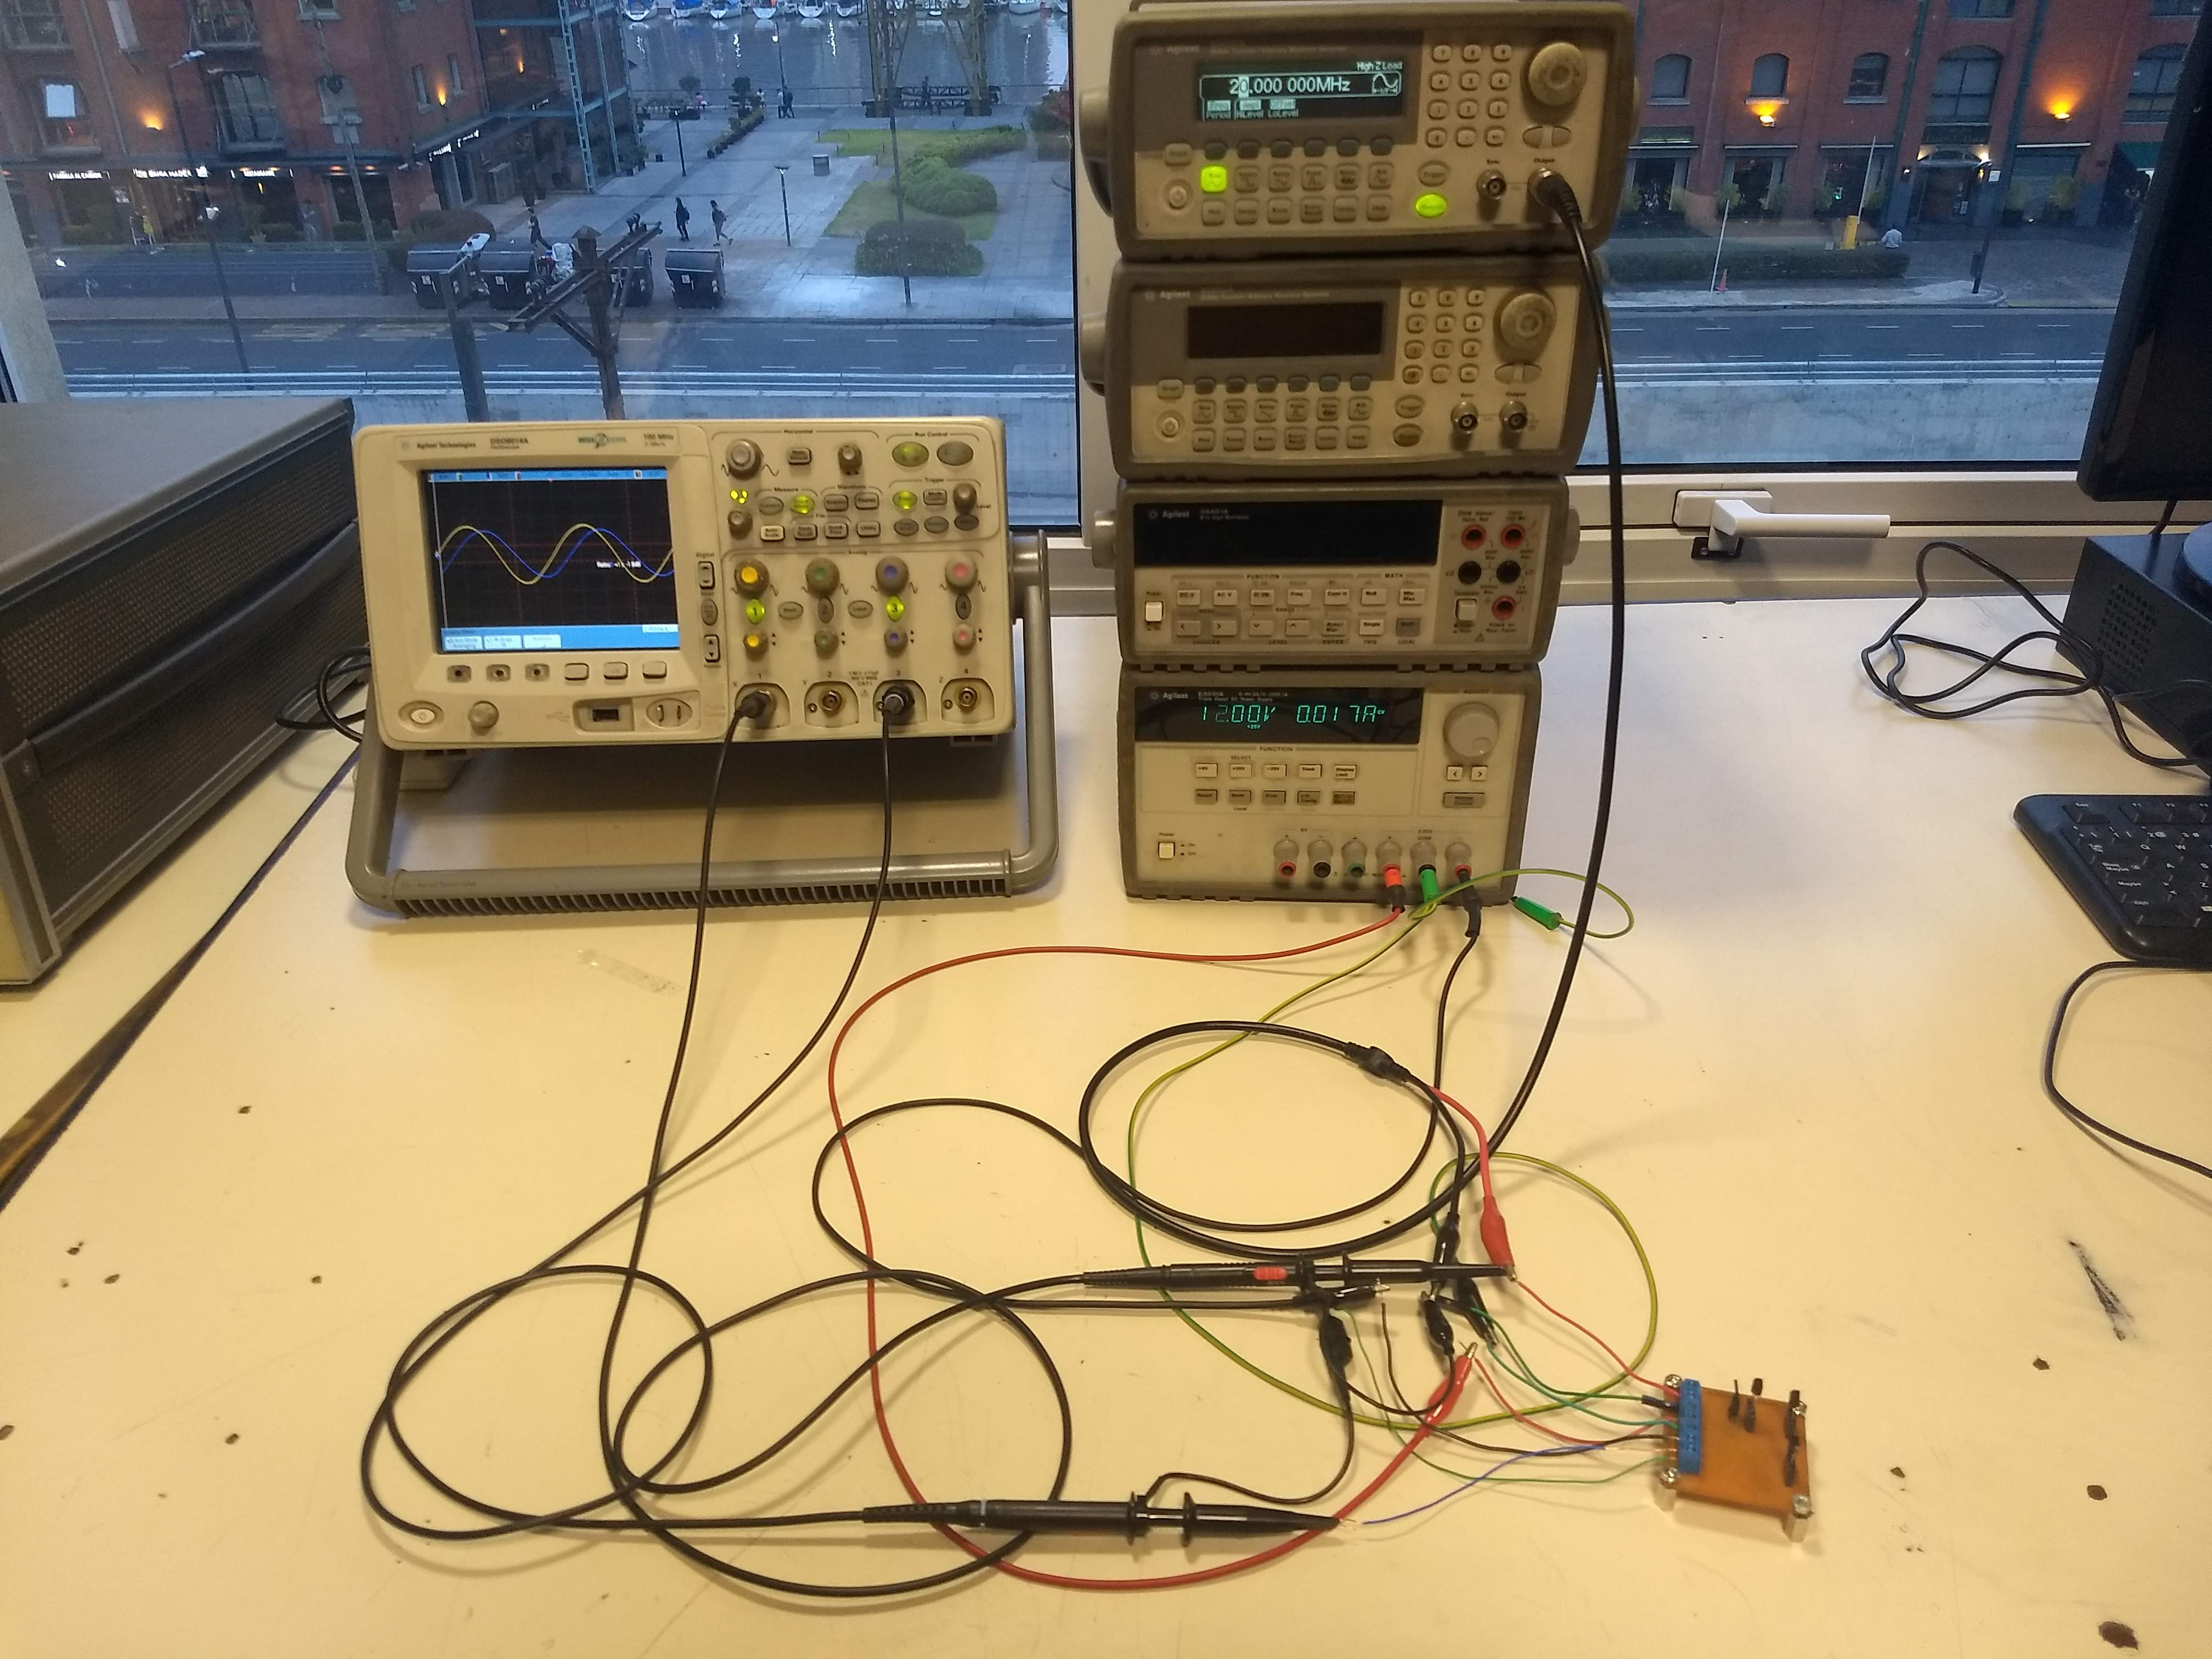
\includegraphics[width=0.4\textwidth, trim={20cm 0 20cm 0}, clip]{Imagenes/Medicion.jpg}
	\caption{Set-up de las mediciones efectuadas.}
	\label{fig:setup}
\end{subfigure}
\caption{Fotografías de la versión física.}
\label{fig:fotos}
\end{figure}

Se colocaron pines hembra para cada transistor, con el mismo objetivo que se colocan zócalos para los distintos tipos de integrados. Además, se colocó un jumper sobre la resistencia $R_g$, de forma que se pueda medir la ganancia de corriente del amplificador y del sistema  con facilidad. Se emplearon resistencias SMD, con tolerancia del $1\%$. Esto se debe a que se buscó la mínima variación posible de las ganancias. Esta decisión queda respaldada por un análisis de Montecarlo efectuado en el programa \textbf{LTSpice}. Se observa en la Figura (\ref{fig:mc-ai1}) como varía la ganancia de corriente del sistema empleando las tolerancias previamente mencionadas. Por otro lado, en la Figura (\ref{fig:mc-ai2}), se efectúa el mismo análisis, pero esta vez con tolerancias del $5\%$. La diferencia entre ambos casos es notable, siendo más estable la primera.
\begin{figure}[H]
\centering
	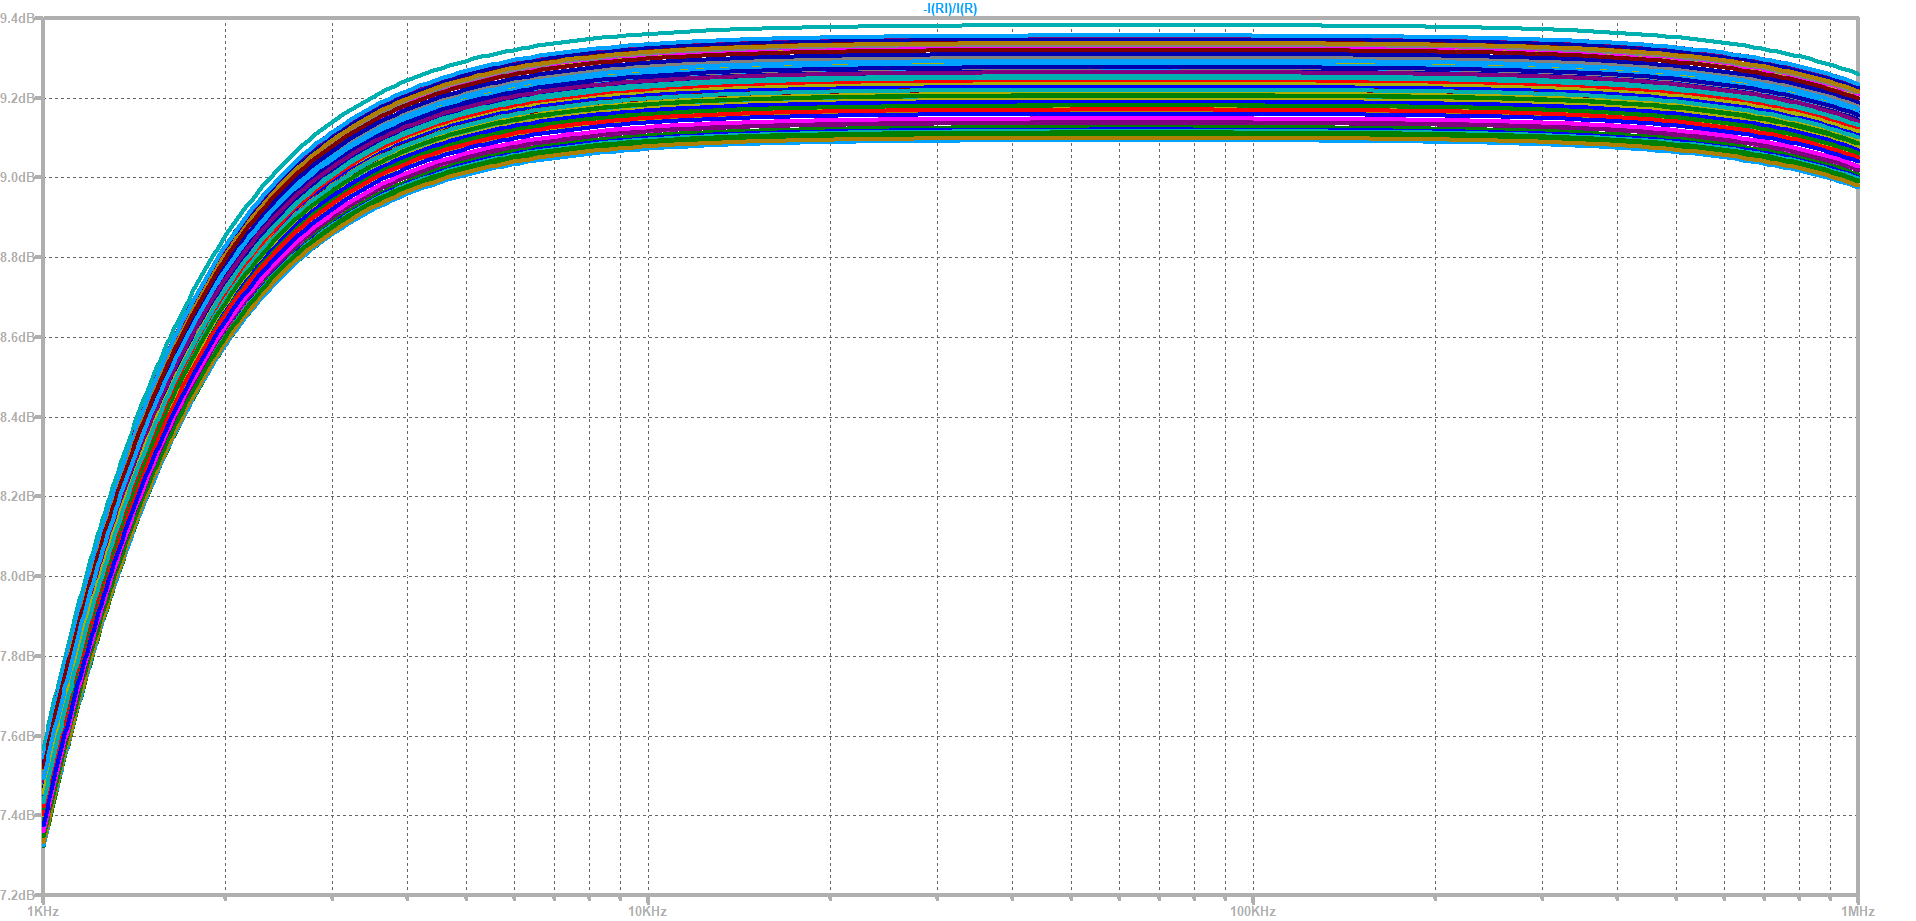
\includegraphics[width=0.6\textwidth]{Imagenes/MC-Ai.png}
	\caption{Montecarlo de la ganancia de corriente con tolerancia del $1\%$.}
	\label{fig:mc-ai1}
\end{figure}
\begin{figure}[H]
\centering
	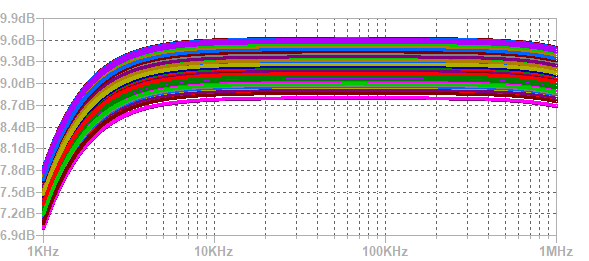
\includegraphics[width=0.6\textwidth]{Imagenes/MC-Ai_2.png}
	\caption{Montecarlo de la ganancia de corriente con tolerancia del $5\%$.}
	\label{fig:mc-ai2}
\end{figure}

\section{Mediciones}
A continuación se procede a analizar los resultados obtenidos de las mediciones sobre el circuito, comparando dichos resultados con los cálculos teóricos y simulados.
\begin{figure}[H]
\centering
\begin{subfigure}{.49\textwidth}
\centering
	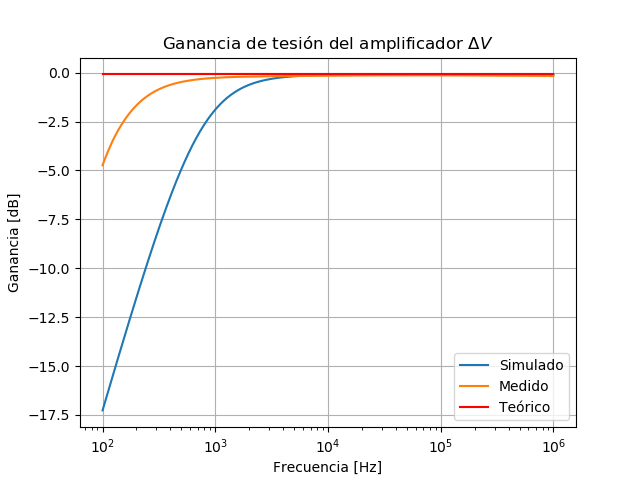
\includegraphics[width=\textwidth]{Imagenes/Av.png}
	\caption{Ganancia de tensión del amplificador.}
	\label{fig:av}
\end{subfigure}
\begin{subfigure}{.49\textwidth}
\centering
	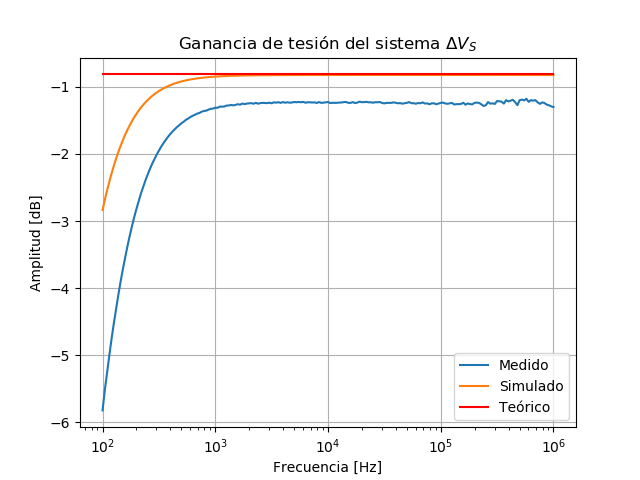
\includegraphics[width=\textwidth]{Imagenes/Avs.png}
	\caption{Ganancia de tensión del sistema.}
	\label{fig:avs}
\end{subfigure}
\begin{subfigure}{.8\textwidth}
\centering
	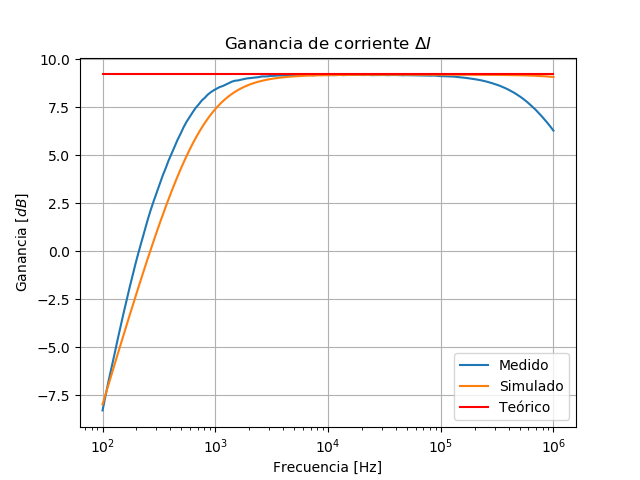
\includegraphics[width=0.6\textwidth]{Imagenes/Ai.png}
	\caption{Ganancia de corriente del amplificador.}
	\label{fig:ai}
\end{subfigure}
\caption{Comparación de ganancias.}
\label{fig:ganancias}
\end{figure}

Se observa de la Figura (\ref{fig:ganancias}) como a frecuencias medias se corresponden los tres valores obtenidos. 
\begin{figure}[H]
\centering
\begin{subfigure}{.49\textwidth}
\centering
	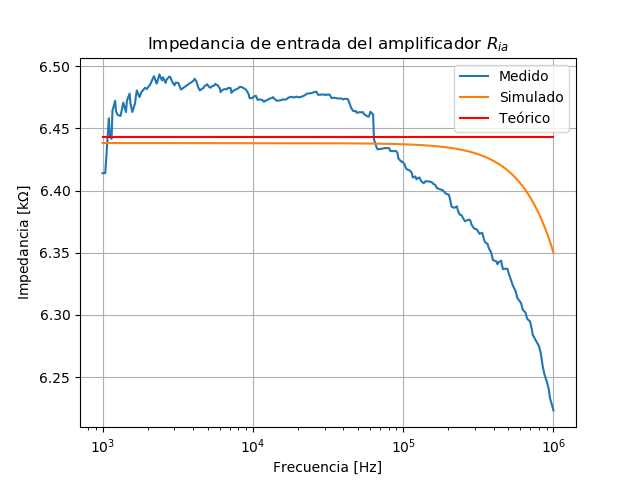
\includegraphics[width=\textwidth]{Imagenes/Ria.png}
	\caption{Impedancia de entrada del amplificador.}
	\label{fig:ria}
\end{subfigure}
\begin{subfigure}{.49\textwidth}
\centering
	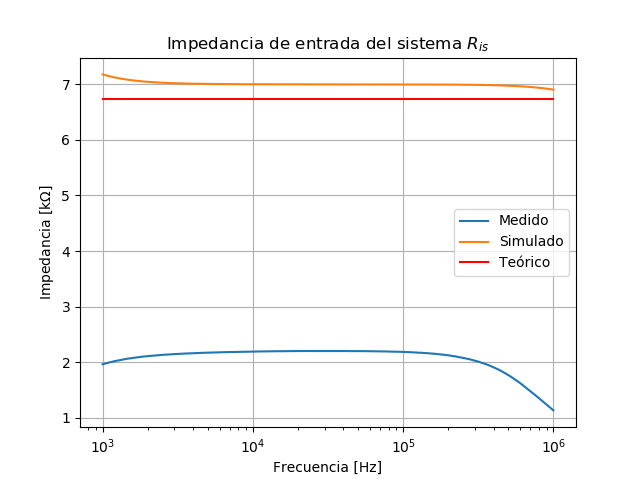
\includegraphics[width=\textwidth]{Imagenes/Ris.png}
	\caption{Impedancia de entrada del sistema.}
	\label{fig:ris}
\end{subfigure}
\caption{Comparación de impedancias de entrada.}
\label{fig:ri}
\end{figure}
\begin{figure}[H]
\centering
	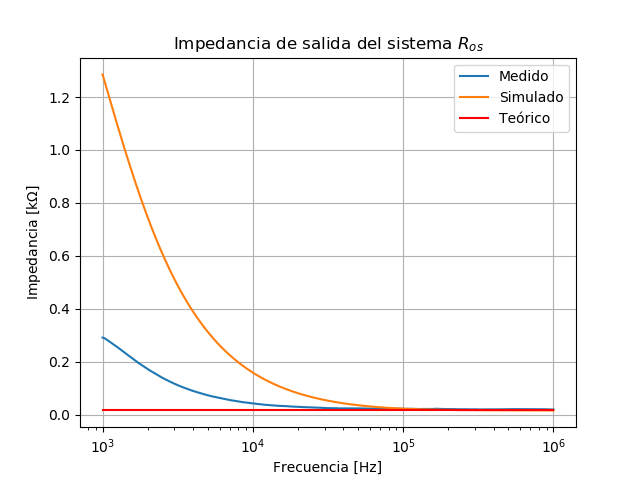
\includegraphics[width=0.5\textwidth]{Imagenes/Ros.png}
	\caption{Comparación de impedancias de salida del sistema}
	\label{fig:ro}
\end{figure}

Cabe aclarar que en las Figuras (\ref{fig:ai}), (\ref{fig:ria}) y (\ref{fig:ris}), tanto las mediciones como las simulaciones presenta una caída a altas frecuencias, alejándose de los valores teóricos. Esto ocurre debido a la presencia de las puntas del osciloscopio con el cual se efectuaron las mediciones. También se debe tener en cuenta que, aunque no se encuentren dichas puntas, para frecuencias más elevadas se presentan polos que generan una caída similar, estos son los conocidos como polos de alta, propios de las capacidades $C_{\mu}$ y $C_{\pi}$ de los transistores. A continuación se presentan simulaciones de los tres parámetros mencionados, comparando sus resultados tanto con como sin punta.
\begin{figure}[H]
\centering
\begin{subfigure}{.47\textwidth}
\centering
	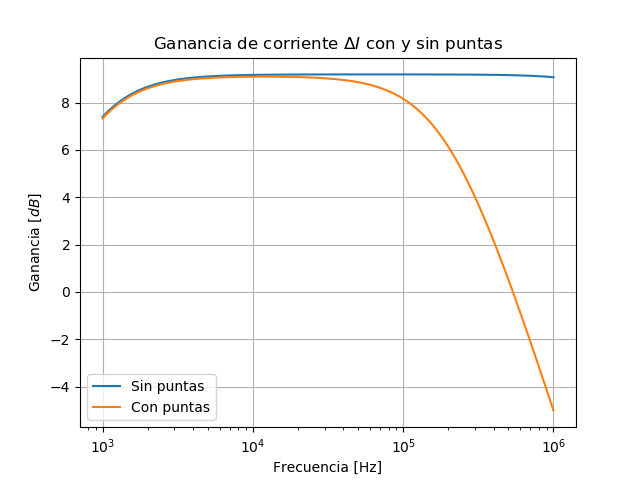
\includegraphics[width=\textwidth]{Imagenes/Ai_cp.png}
	\caption{Ganancia de corriente.}
	\label{fig:ai-cp}
\end{subfigure}
\begin{subfigure}{.47\textwidth}
\centering
	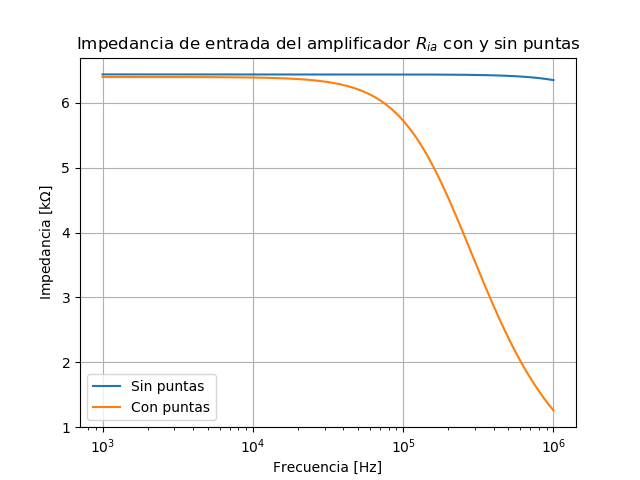
\includegraphics[width=\textwidth]{Imagenes/Ria_cp.png}
	\caption{Impedancia de entrada del amplificador.}
	\label{fig:ria-cp}
\end{subfigure}
\begin{subfigure}{.5\textwidth}
\centering
	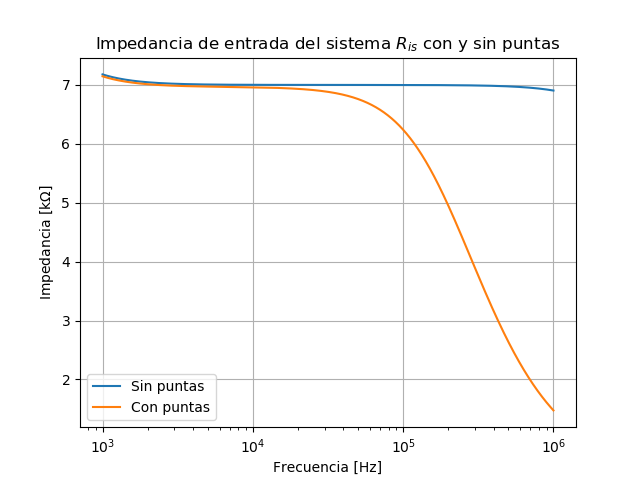
\includegraphics[width=1\textwidth]{Imagenes/Ris_cp.png}
	\caption{Impedancia de entrada del sistema.}
	\label{fig:ris-cp}
\end{subfigure}
\caption{Comparación de simulaciones con y sin punta.}
\label{fig:cpvssp}
\end{figure}

\section{Conclusiones} \label{sec:conclusiones}
Dado que se optó por confeccionar una configuración Darlington, era esperable obtener una ganancia de corriente alta. Se pretendía obtener $\Delta I \approx h_{fe1} h_{fe2} = 40000$. Como se demostró en la Tabla (\ref{tab:resultados}) y en la Figura (\ref{fig:ai}), esto no resultó así, sino que se obtuvo una ganancia mucho más baja. Una de las soluciones posibles consiste en aumentar el valor de la resistencia $R_B$, adecuando también toda la polarización a esto, ya que si se toma $R_B \rightarrow \infty$, se obtiene $\Delta I \approx 36 \ dB$. Esto no resultó posible de efectuarse ya que los componentes son limitados. 

Con lo dicho anteriormente, se contempla retirar la resistencia $R_S$ de la fuente de corriente y colocarla en serie con la resistencia $R_B$. De esta forma, se logra incrementar la resistencia deseada, ya que se presentan dos impedancias de $6.8 \ k\Omega$ en serie. A costo de esto, se obtiene una fuente de corriente cuya $I_D$ es igual al valor $I_{DSS}$. Si bien esta corriente aumenta, este tipo de fuente no es estable, ya que dicho valor no lo es, provocando variaciones en los parámetros del sistema.

Si bien se obtuvo una buena ganancia de tensión del amplificador, es decir, el circuito resulta ser un buen seguidor de tensión, dado que su impedancia de entrada no resulta mucho mayor a la del generador, el sistema no cuenta con dicha cualidad. Esto, nuevamente se puede solucionar aumentando $R_B$. Si se realiza el mismo análisis que se efectuó previamente para el caso de la ganancia de corriente, se obtiene $R_{ia} \rightarrow \infty$, lo que concluye en $\Delta V = \Delta V_S$. En otras palabras, se está buscando efectuar una adaptación de las impedancias. Si bien esto no se puede lograr con los componentes disponibles, lo que sí se obtuvo es una baja impedancia de salida, lo que permite una buena adaptación en caso de conectar otro sistema a la salida de este. 

Por otro lado, es posible afirmar que la polarización resulta estable, ya que se logró efectuarla mediante una fuente de corriente. Una alternativa aún mejor al circuito desarrollado, se basa en polarizar ambos transistores mediante el uso de fuentes de corriente. Si bien se cuenta con un diodo y un transistor NPN que no se han utilizado, no se poseen los componentes suficientes para realizar dicha disposición. Mínimamente se requeriría un diodo y dos resistencias más para efectuar una fuente simple compensada. También se destaca que se pudo haber colocado un diodo entre el colector y el emisor de $Q_2$. Este tipo de configuración es utilizada para trabajar con potencias altas. Dado que este enfoque no es de interés, se reserva dicho componente.

Finalmente, se destaca un último punto, el cuál consiste en el ancho de banda del circuito. Se pudo corroborar, mediante observaciones en el laboratorio, que si se emplea el sistema como seguidor de tensión, dicha variable es sumamente grande. Analizando que, limitado por la frecuencia máxima del generador, a $20 \ MHz$ se presenta una atenuación menor a $2 \ dB$. Esto muestra que, empleando el circuito como seguidor de tensión, este posee un ancho de banda superior que al de varios operacionales comerciales, como por ejemplo lo son el \href{http://www.ti.com/lit/ds/symlink/tl082-n.pdf}{TL082} con $3 \ MHz$, \href{http://www.ti.com/lit/ds/symlink/lm833.pdf}{LM833} con $10 \ MHz$ y el \href{http://www.ti.com/lit/ds/symlink/lm741.pdf}{LM741} con $1.5 \ MHz$.
\end{document}